\documentclass[oneside]{book}
\usepackage{fullpage}
\usepackage{graphicx}
\usepackage[numbers,sort&compress]{natbib}
\usepackage{pdflscape}

\usepackage{titlesec}

%\titleformat{\chapter}[display]
%  {\normalfont\LARGE\bfseries}{\chaptertitlename\ \thechapter}{12pt}{\LARGE}

%\renewcommand{\chaptername}{}

\titleformat{\chapter}
	{\normalfont\LARGE\bfseries}
	{\thechapter} {0.5em} {}

\titlespacing*{\chapter}{0pt}{0pt}{10pt}

\begin{document}

%\title{Mirrorshades}
\title{Mirrorshades: Phase 1 Investigation}
\author{CJ Davies}

\maketitle

%=========================================================================================================
%=========================================================================================================

\chapter{The Case for Mobile XR}
This investigation compares two scenarios for interaction with a real location \& a corresponding virtual location.

\begin{enumerate}
	\item \textbf{Stationary scenario} - interacting with the virtual location from a fixed real location, then subsequently interacting with the real location.
	\item \textbf{Mobile scenario} - using the Mirrorshades platform to interact with both the real location \& the corresponding virtual location in tandem, whilst moving around both environments.
\end{enumerate}

The locations in question are St Salvator's chapel \& a virtual reconstruction of the chapel as it stood in 1450-1460. The stationary scenario is representative of how virtual reality technologies, including both CAVEs \& HMDs, have previously been used for dissemination of virtual reality content in cultural heritage contexts~\cite{Roussou2002} \& thus this investigation serves to compare Mirrorshades with previous applications virtual reality content to these contexts.

\section{Process}
\begin{itemize}
	\item Participants complete a pre-task questionnaire, which provides calibration for their subsequent responses by enquiring about age, gender identity, previous experience with VR hardware \& previous interactions with either the real or virtual chapel. This questionnaire is included as Appendix \ref{pre_task_questionnaire}.
	
	\item Participants familiarise themselves with the experience of using the Oculus Rift DK1 HMD \& the Xbox 360 controller by interacting with the `Tuscany demo' prepared \& maintained by the Oculus VR team. This is performed from a seated position.
	
	\item Participants complete the stationary scenario.
	
	\item After completing the stationary scenario, participants complete the System Usability Scale (SUS)~\cite{Brooke1996} questionnaire, included as Appendix \ref{sus} \& a 12-item questionnaire, included as Appendix \ref{12_questions}.
	
	\item Participants complete the mobile scenario.
	
	\item After completing the mobile scenario, participants complete the SUS questionnaire \& the 12-item questionnaire again.
	
	\item Finally, the participant is engaged in a short structured interview. Interview prompts are included as Appendix \ref{interview_questions}.
\end{itemize}

In addition to SUS, the 12-item questionnaire \& the structured interview, quantitative data is logged by the Mirrorshades platform when a participant is interacting with virtual content in the first scenario \& at all times during the second scenario.

\section{The Scenarios}
Both scenarios that participants complete for this investigation are designed to mimic the style of exploration \& interaction that visitors to the chapel display, which was observed over several occasions. Visitors enter the chapel from the North/West corner then proceed to walk Eastwards along the nave, pausing to look around after passing through the rood screen, before continuing along the nave toward the altar. Visitors pause in front of the alter upon reaching the end of the pews \& then walk North toward the tomb where they pause again to inspect it. Participants are instructed to imagine that they are performing a similar visit to the chapel \& to follow a similar path, pausing after the rood screen, at the end of the pews \& in front of the tomb. Participants are shown the map included as figure \ref{chapel_path} to explain the scenario better.

In the stationary scenario, participants interact with the virtual chapel using the Rift \& Xbox controller, whilst in a sitting position. After completing the path, they remove the headset \& then walk the same path in the real chapel. This scenario alludes to how virtual reality technologies have previously been applied to cultural heritage situations, allowing visitors to experience a virtual reality reconstruction or reimagination of the real environment from a fixed position \& with their view of the real environment wholly occluded by their view of the virtual environment.

In the mobile scenario, participants wear the HMD, hold the Xbox controller in their right hand \& the smartphone in their left, with the laptop \& battery pack in a satchel worn over the right shoulder. They then walk the same path, but this time with the ability to transition at any time between viewing the real environment \& the virtual environment from the same vantage point.

In this first investigation phase, only one transition is available to participants. Preliminary experiments involving the researchers' colleagues that allowed hard transitions, linear interpolated transitions \& analogue selectable opacity, indicated that the linear interpolated transition was preferred to either the hard transition or the analogue selectable opacity \& thus this is the transition available to participants in this first phase investigation.

\begin{figure}[h]
	\begin{center}
		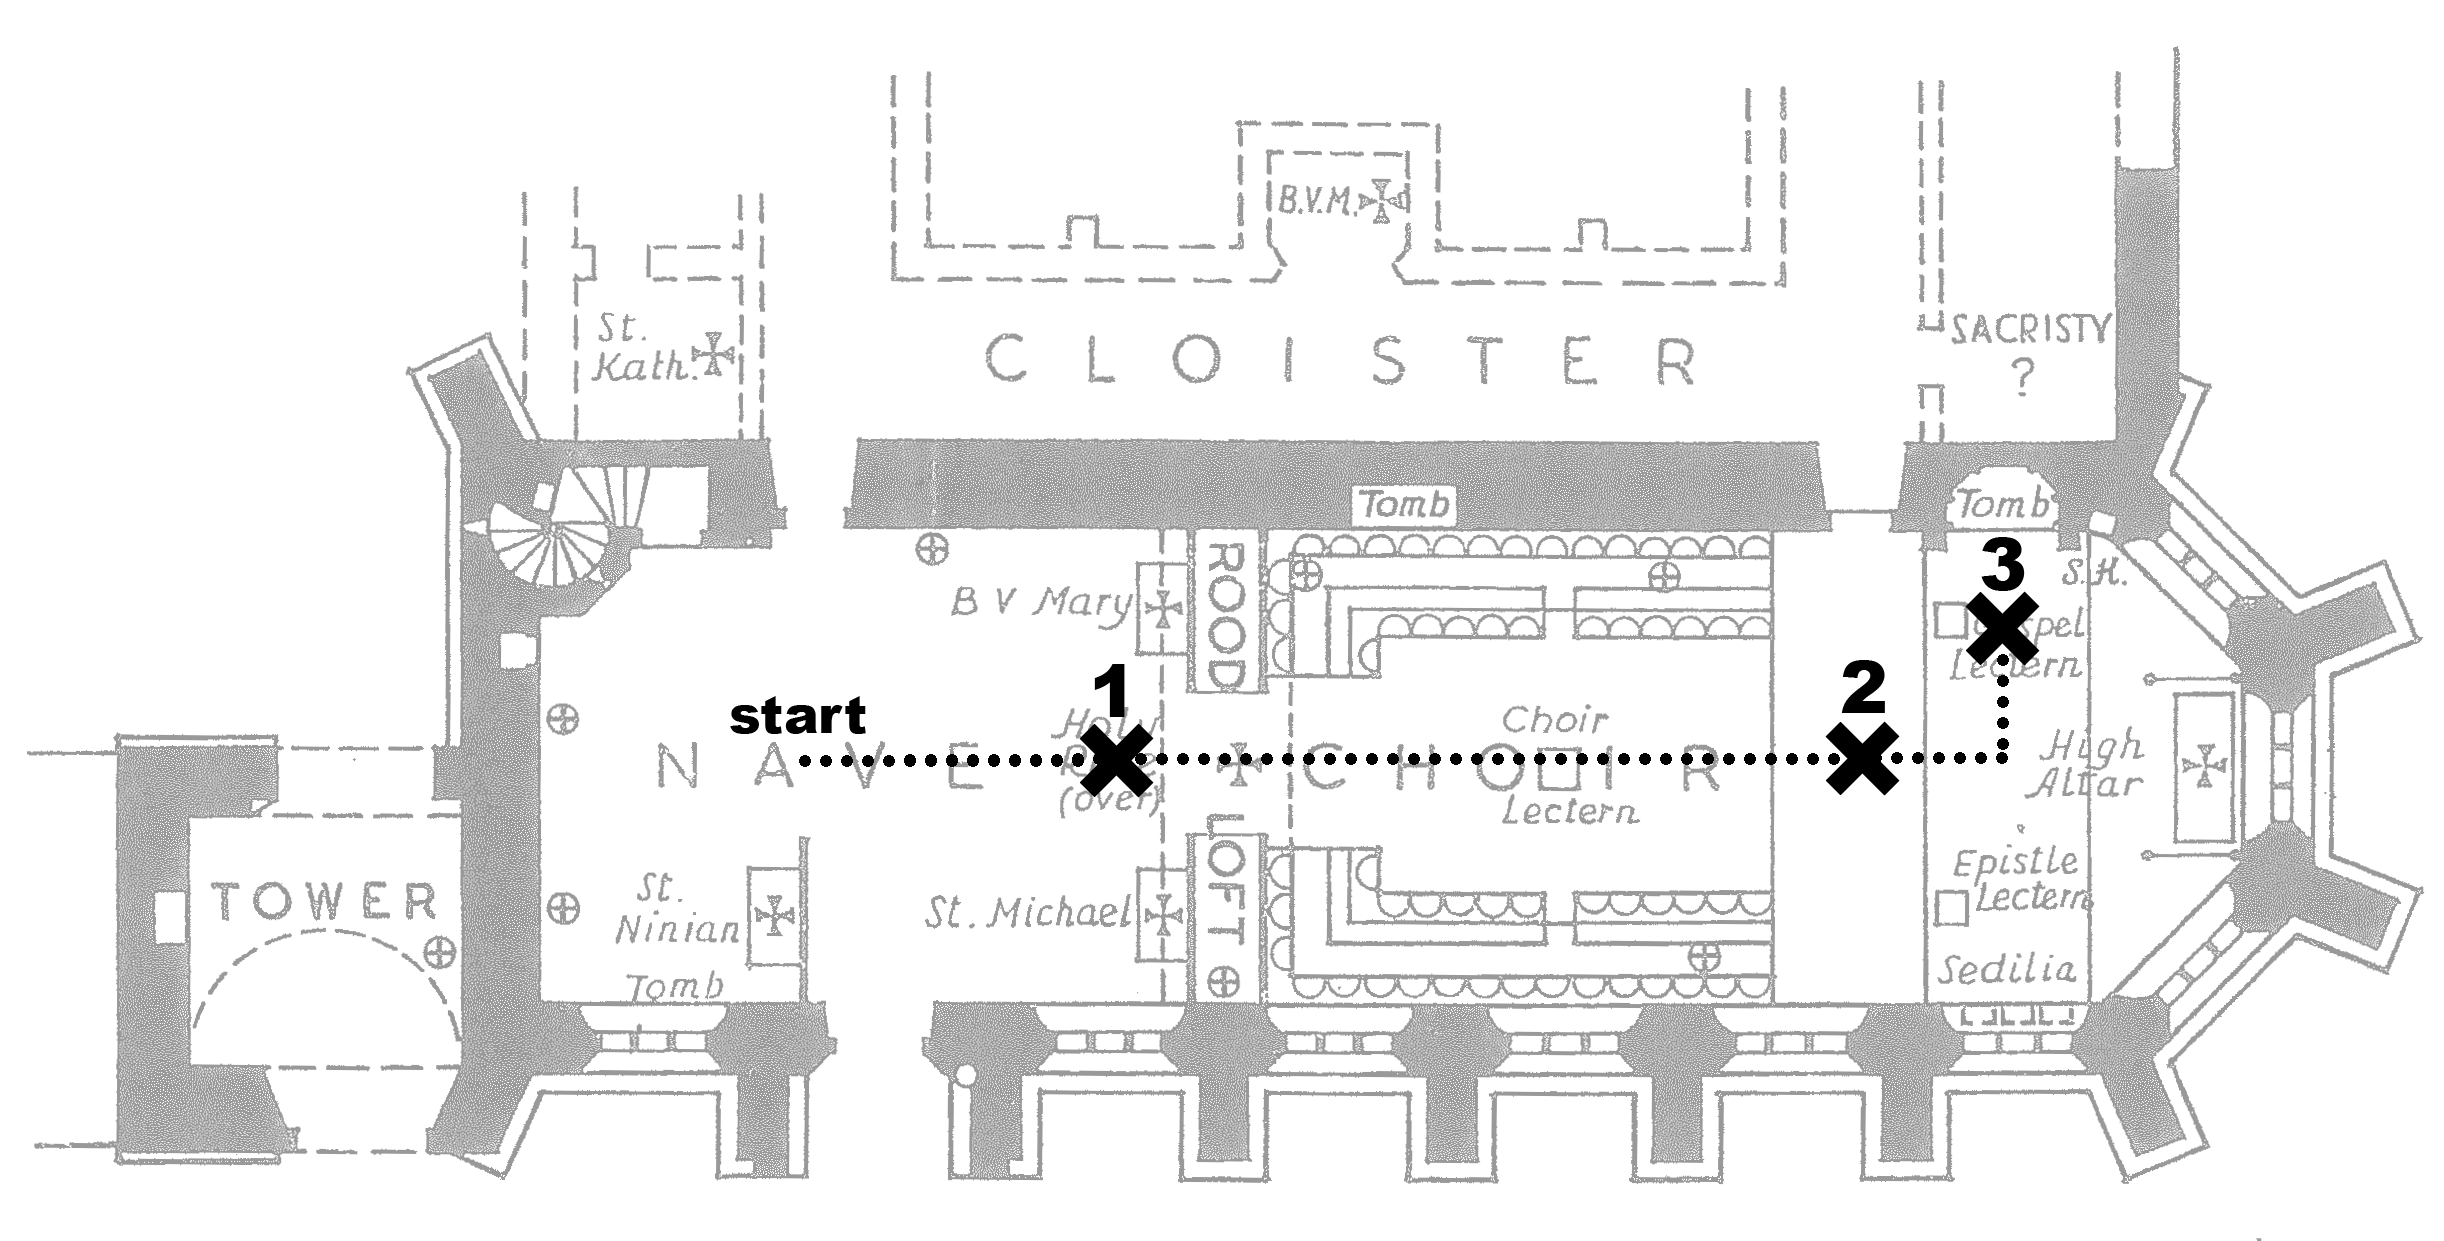
\includegraphics[width=\linewidth]{images/chapel_path.png}
		\caption{The path \& positions within the chapel that participants are instructed to attend to.}
		\label{chapel_path}
	\end{center}
\end{figure}

\section{Hypotheses}
The aim of the mobile scenario is to improve participant engagement with \& understanding of the relationships between the real \& virtual environments, by addressing the problems of spatial \& temporal separation inherent with the `traditional' stationary scenario, by imparting upon the participant the ability to transition between equivalent vantage points within the real \& virtual environments at will.

While we expect participants to report that the mobile scenario does indeed allow them to better compare \& contrast the real \& virtual environments, identify differences between the real \& virtual environments \& gain a better understanding of how the real \& virtual environments relate to each other, we expect some participants to report that having to `split' their attention between the two environments in the mobile scenario leads to lessened engagement \& understanding \& that the visual quality of the real view through the headset/cameras leads to some participants preferring to interact with the real environment without the headset.

We expect the cumbersome nature of the mobile scenario \& the reduced quality of viewing the real environment via the headset/cameras to have a noticeable effect upon participants movement (both position \& head orientation) in the mobile scenario.

Addressing these issues, such that participants don't find viewing the real through the headset to be such a reduction in quality compared to just seeing real, such that participants feel as though they can move \& look around themselves as much in the mobile scenario as in the stationary scenario \& such that participants transition between real \& virtual at any time instead of avoiding transitions in situations in which they think that they will be unpleasant/jarring, is key \& what the next stage will focus on.

%Engagement with individual environments will be lessened
%Engagement with both environments will be increased
%So for tasks where real time comparison \& contrast is required, this is good

\subsection{SUS}
SUS scores for the mobile scenario are expected to average lower than those for the stationary scenario, due to the cumbersome nature of the platform when performing the mobile scenario; during the stationary scenario, participants are seated, whilst during the mobile scenario they are required to carry a satchel over one shoulder \& hold a smartphone in their left hand. Participants who are able to overcome this cumbersomeness are expected to respond more favourably to the mobile scenario than those who cannot overcome it.

\subsection{12-item Questionnaire}
\begin{itemize}
	\item Participants will find it easier to compare \& contrast real \& virtual environments in the mobile scenario than in the stationary scenario (q2)
	\item Participants will experience a greater  sense of `being in' the virtual environment in the mobile scenario than in the stationary scenario (q4, due to physical movement/embodiment)
	\item Participants will have a greater sense of `being in the past' in the mobile scenario than in the stationary scenario (q7)
	\item Participants will maintain greater awareness of both real \& virtual environments in the mobile scenario than in the stationary scenario (q5)
%	\item Participants will notice more differences between real \& virtual environments in the mobile scenario than in the stationary scenario (q10)
	\item Participants will gain a better understanding of what the chapel was like in the past in the mobile scenario than in the stationary scenario (q12)
\end{itemize}

\subsection{Log data}
\begin{itemize}
	\item Head movement (pitch \& yaw) will be more restricted in the mobile scenario compared to the stationary scenario
	\item Aversion to looking around (even at real) when moving in the mobile scenario
	\item Head movements will be larger discrete changes in the stationary scenario compared to the mobile scenario
	\item Tendency to only look at virtual when looking around
\end{itemize}

\subsection{Interviews}
\begin{itemize}
	\item mobile scenario makes it easier to spot differences
	\item mobile scenario reveals differences that stationary didn't
	\item stationary does not reveal differences that mobile doesn't
	\item mobile scenario is preferred \& is user-reported as 'more engaging'
\end{itemize}

%=========================================================================================================

\section{Results}

\subsection{Pre-task Questionnaire}

For n=5 ages ranged from 21-26, 3x female \& 2x male, all reported previous experience using a games console controller, 1x reported previous use of a HMD, 2x reported having previously visited the chapel, none had previously interacted with the virtual chapel model.

%0 = false
%1 = true

%+------+------+------+------+------+------+------+
%| id   | q1   | q2   | q3   | q4   | q5   | q6   |
%+------+------+------+------+------+------+------+
%|    1 |   25 | f    |    1 |    1 |    1 |    0 |
%|    2 |   21 | m    |    1 |    0 |    0 |    0 |
%|    3 |   26 | m    |    1 |    0 |    0 |    0 |
%|    4 |   22 | f    |    1 |    0 |    1 |    0 |
%|    5 |   23 | f    |    1 |    0 |    1 |    0 |
%+------+------+------+------+------+------+------+

\pagebreak

\subsection{SUS}

\begin{figure}[h]
	\begin{center}
		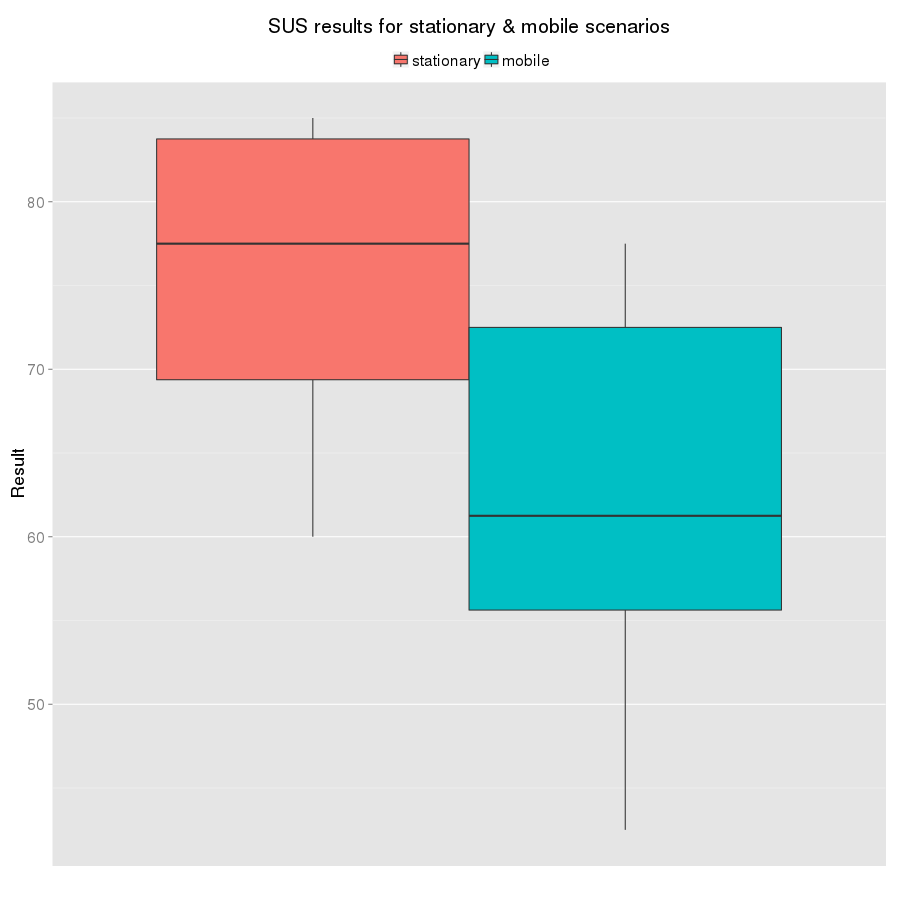
\includegraphics[width=0.7\linewidth]{images/sus.png}
		\caption{SUS results.}
		\label{sus}
	\end{center}
\end{figure}

As expected, the SUS scores for the mobile scenario are lower than those of the stationary scenario, although not drastically so. Furthermore, although scoring lower on SUS, the mobile scenario came out above the stationary scenario when looking at the results of q8 in the 12-item questionnaire which asked participants if they thought they would have preferred a conventional computer monitor.

\pagebreak

\subsection{12-item Questionnaire}

\begin{figure}[h]
	\begin{center}
		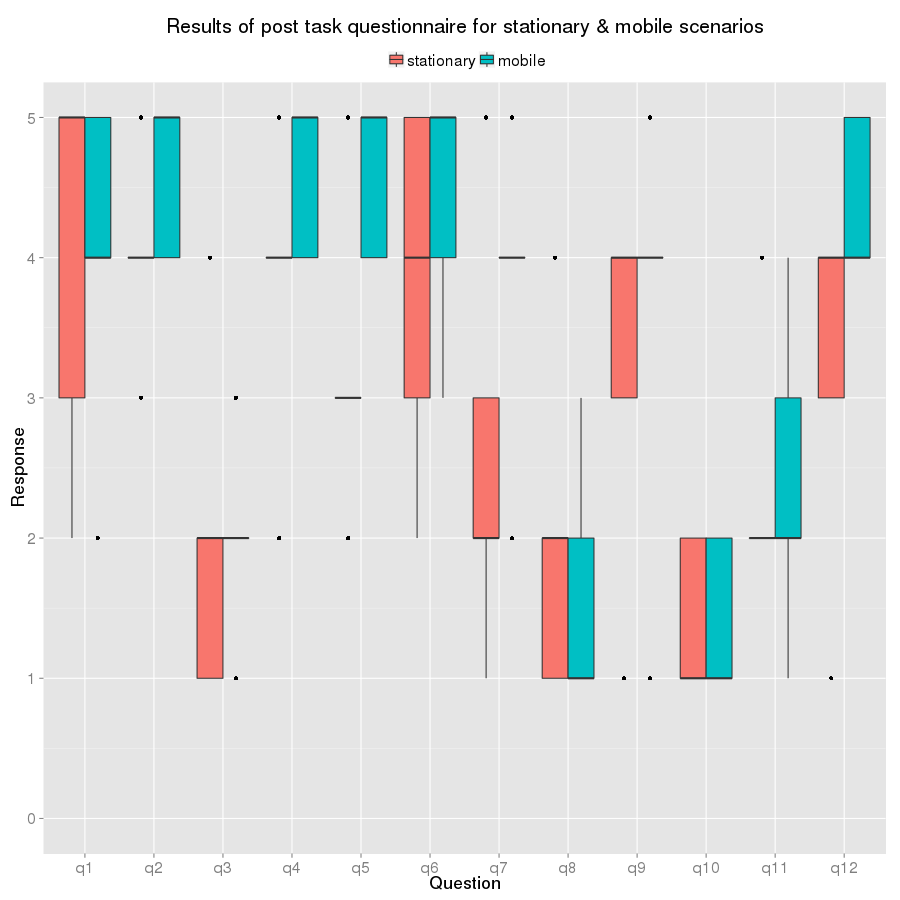
\includegraphics[width=0.9\linewidth]{images/post_task_questionnaire_boxplot.png}
		\caption{12-item questionnaire results.}
		\label{12-item_boxplot}
	\end{center}
\end{figure}

The hypotheses seem to hold, in particular;

\begin{itemize}
	\item \textit{Participants will maintain greater awareness of both real \& virtual environments in the mobile scenario than in the stationary scenario} is supported by the responses to q5
	\item \textit{Participants will have a greater sense of `being in the past' in the mobile scenario than in the stationary scenario} is supported by q7 (thanks to embodiment?)
	\item \textit{Participants will gain a better understanding of what the chapel was like in the past in the mobile scenario than in the stationary scenario} is supported by q12
\end{itemize}

It is worth highlighting the responses to q10 in relation to those to q2. Participants reported finding it easier to compare features from the past \& present (q2) during the mobile scenario, however did not report a difference between not noticing differences between the real \& virtual environments (q10).

\subsection{Log data}

%Amongst the details captured by the automatic logging, the relationships revealed between movement, head orientation \& when participants transitioned between real \& virtual are the most interesting.


%comparing the plots for
%	distance moved against time for stationary scenario
%	\&
%	pitch \& yaw against time for stationary scenario
	
%against
%	distance moved against time for mobile scenario
%	\&
%	pitch \& yaw against time for mobile scenario

%supports the hypotheses that
%	head movement will be more restricted in the mobile scenario compared to the stationary scenario
		
%	in the mobile scenario participants seem to only look around
%		when standing still
%		when looking at virtual
%	the fact that participants didn't look around themselves when moving \& looking at real would seem to imply that participants did not feel comfortable enough when moving with the headset on to engage fully with their real environment \& instead had to focus all of their attention on looking straight ahead in the direction they were walking

***stats here (see R output files)

%=========================================================================================================

\begin{landscape}
	\begin{figure}[h]
		\begin{center}
			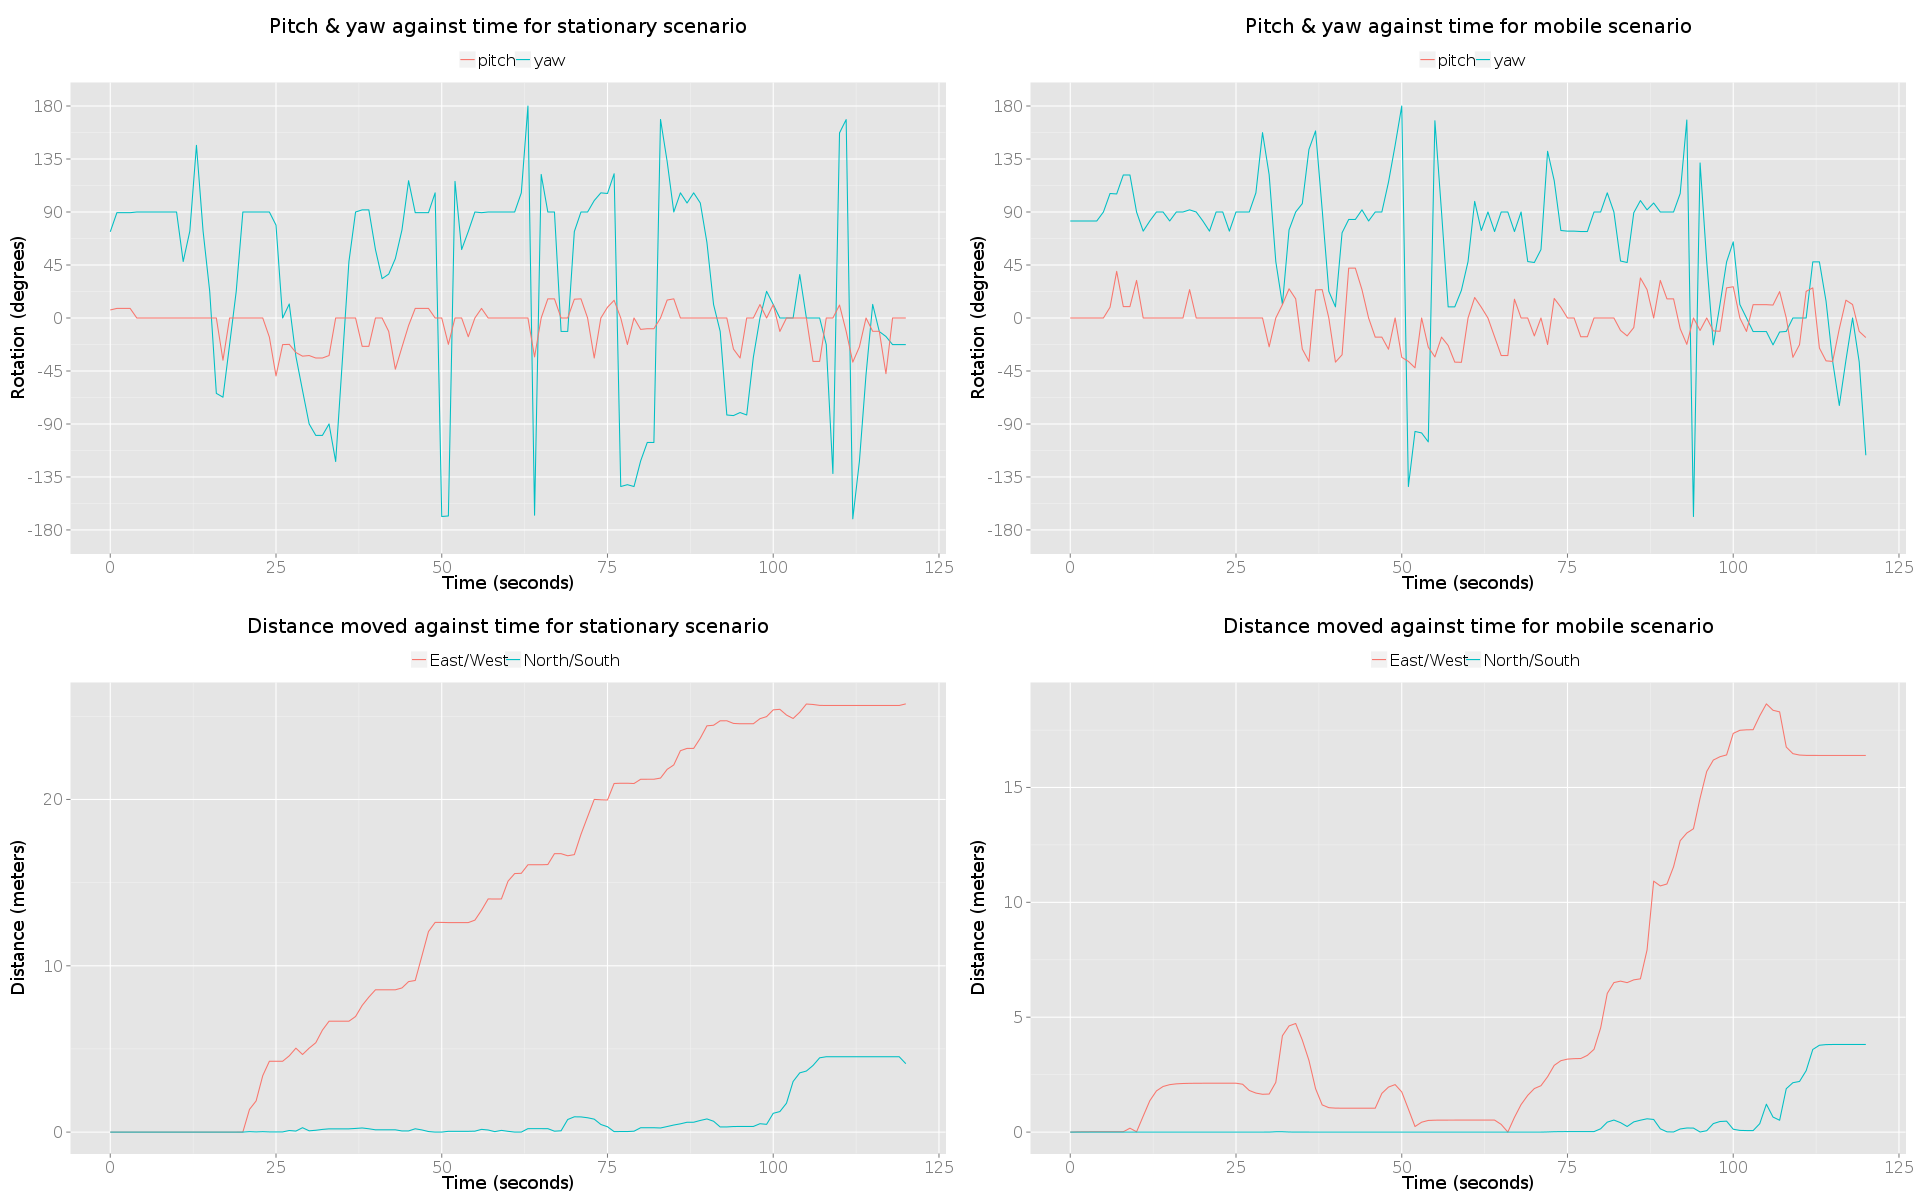
\includegraphics[width=\linewidth]{images/24072014_1200_4up.png}
			\caption{Participant 1}
			\label{participant_1_4up}
		\end{center}
	\end{figure}
\end{landscape}

\begin{figure}[h]
	\begin{center}
		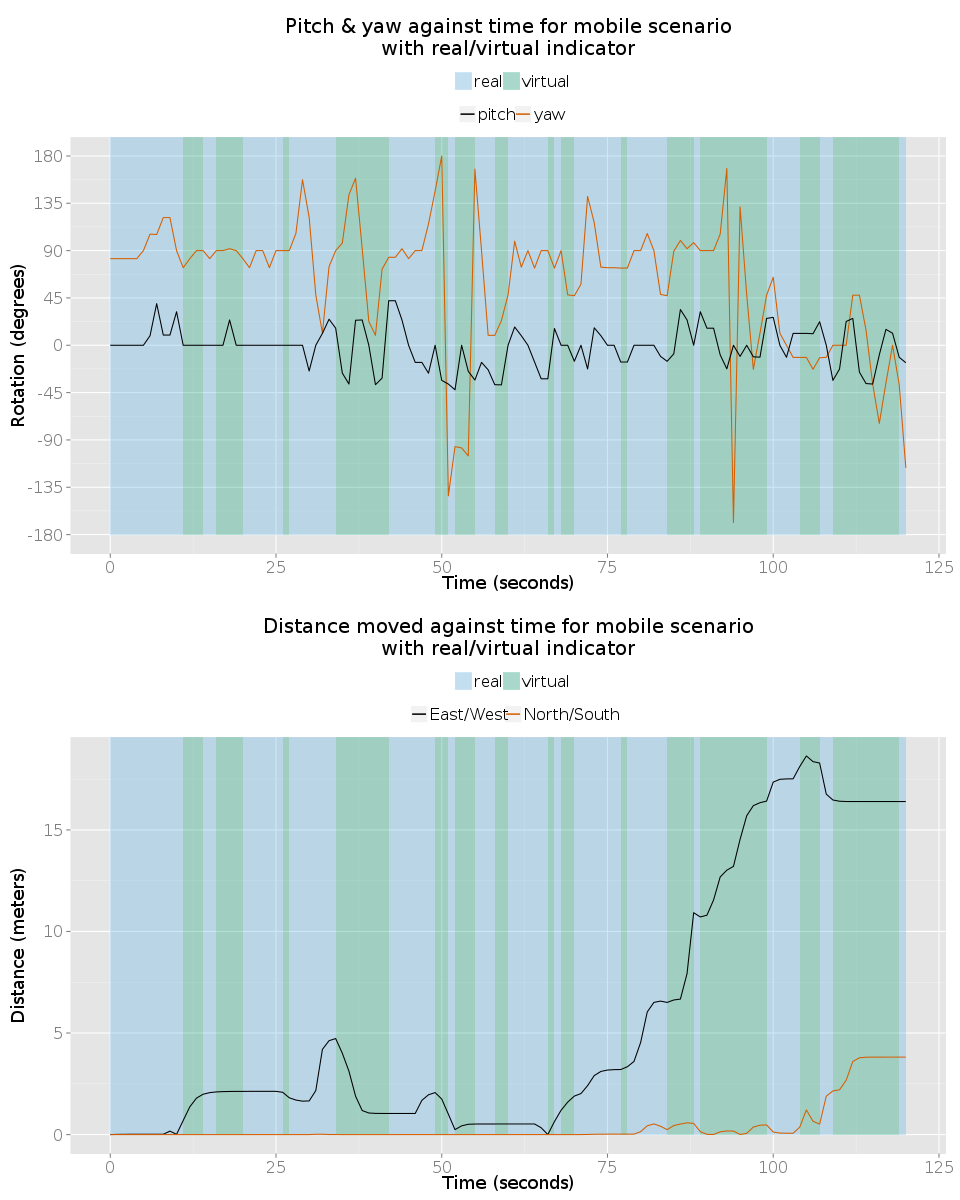
\includegraphics[width=\linewidth]{images/24072014_1200_2up.png}
		\caption{Participant 1}
		\label{participant_1_2up}
	\end{center}
\end{figure}

%=========================================================================================================

\begin{landscape}
	\begin{figure}[h]
		\begin{center}
			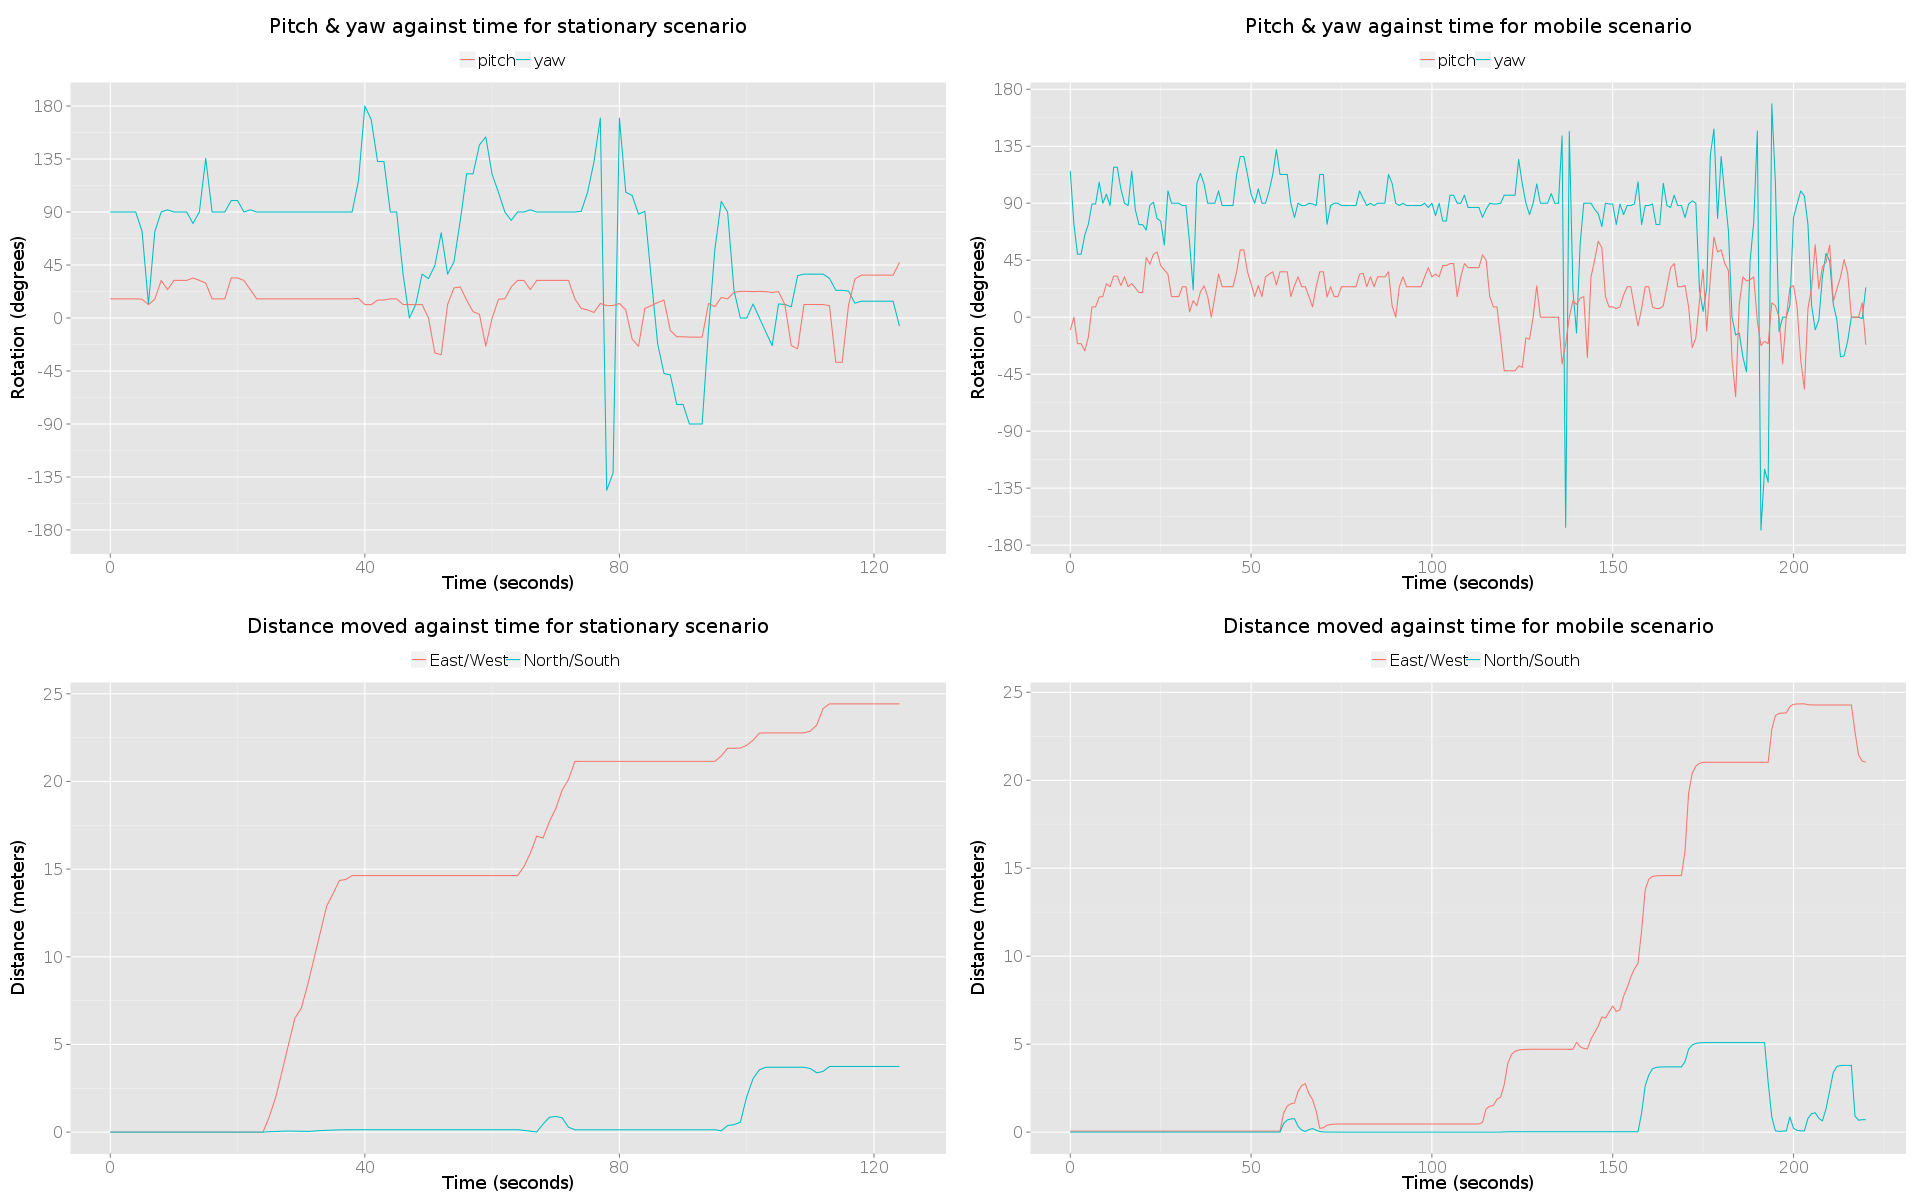
\includegraphics[width=\linewidth]{images/25072014_1300_4up.png}
			\caption{Participant 2}
			\label{participant_2_4up}
		\end{center}
	\end{figure}
\end{landscape}

\begin{figure}[h]
	\begin{center}
		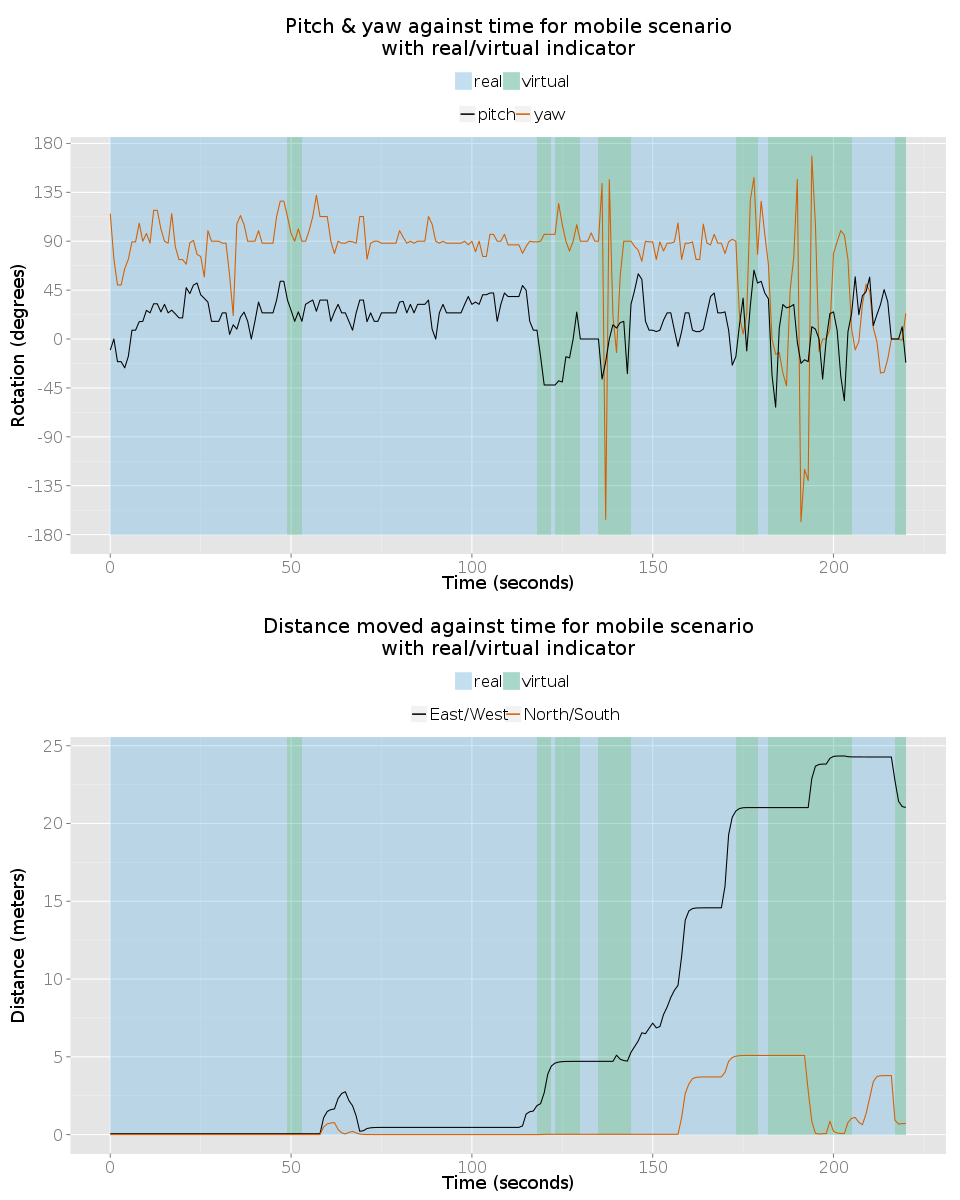
\includegraphics[width=\linewidth]{images/25072014_1300_2up.png}
		\caption{Participant 2}
		\label{participant_2_2up}
	\end{center}
\end{figure}

%=========================================================================================================

\begin{landscape}
	\begin{figure}[h]
		\begin{center}
			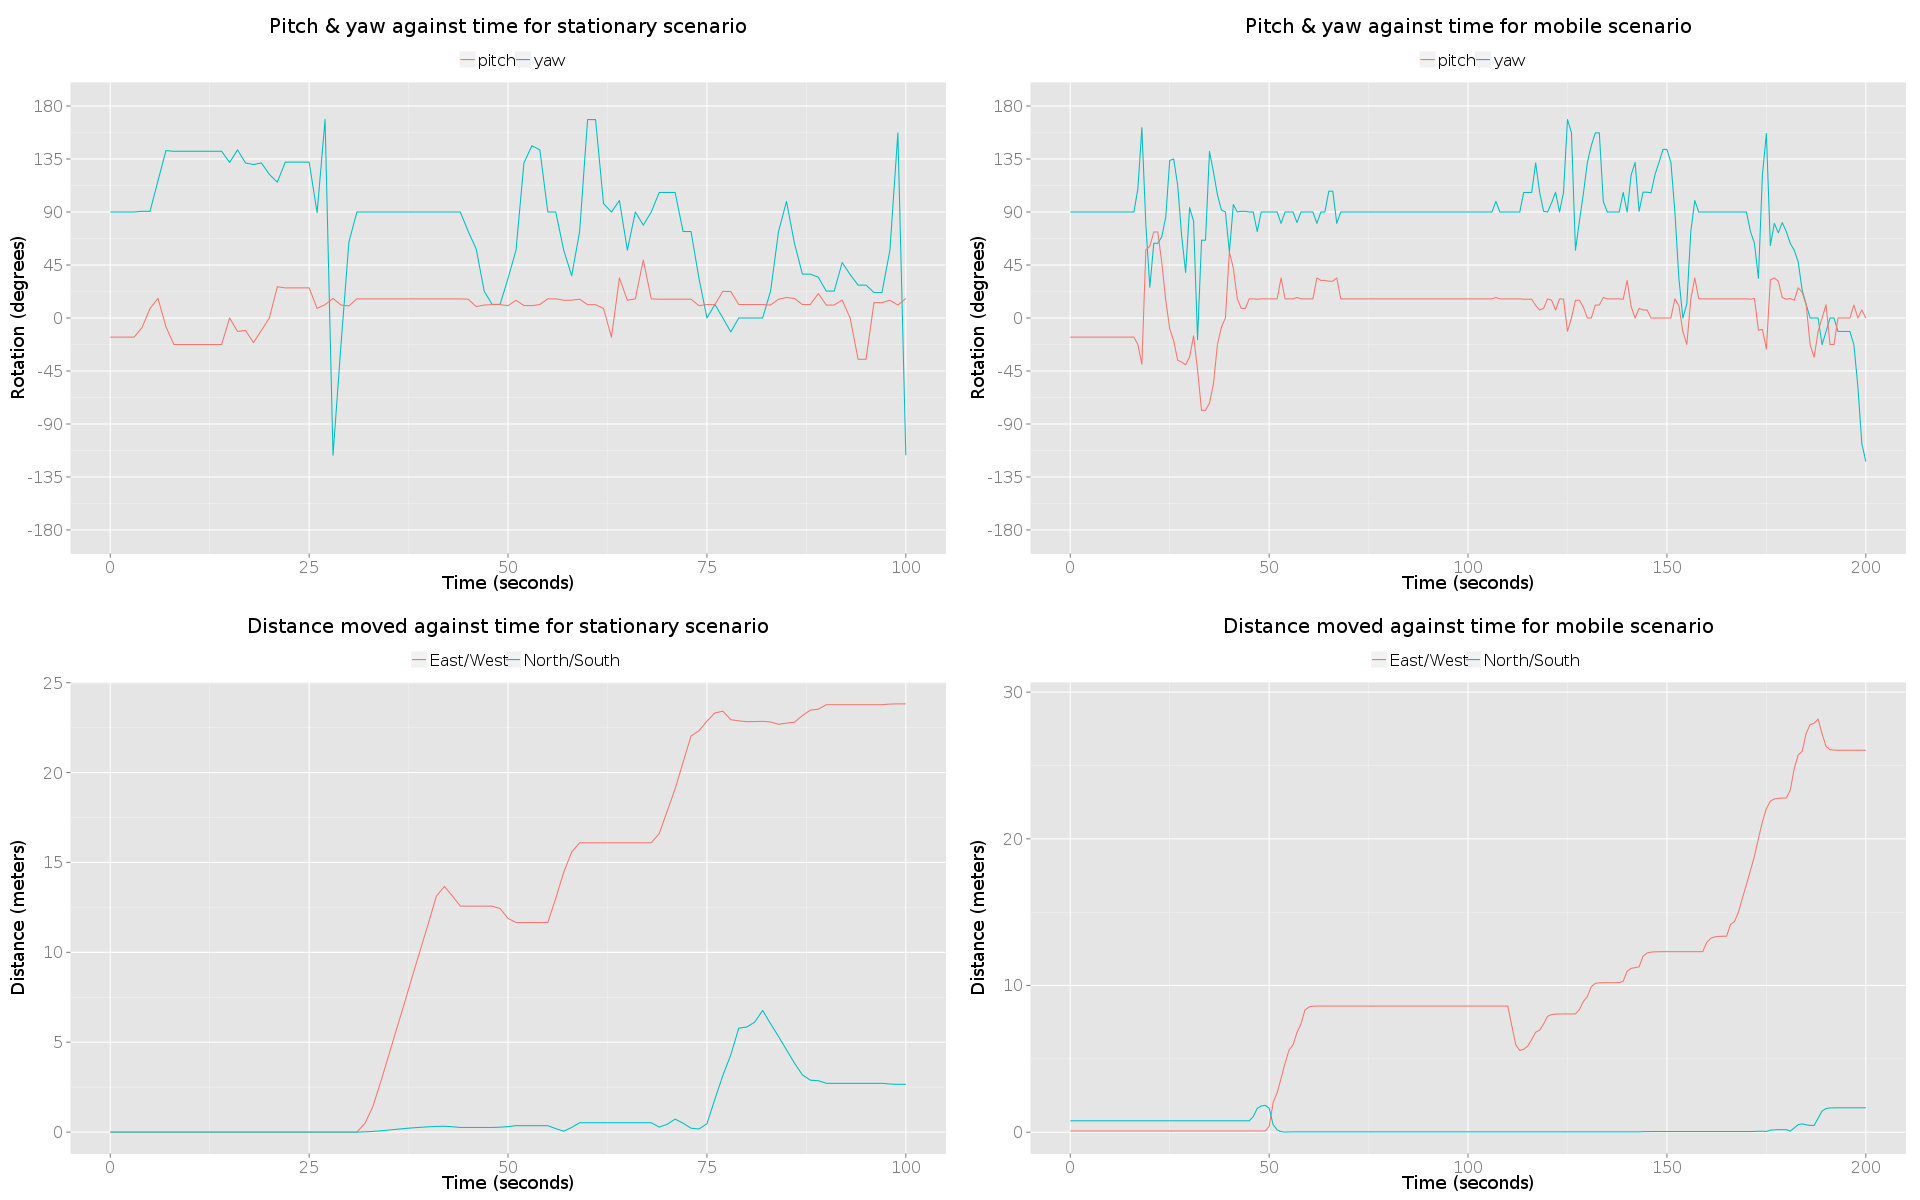
\includegraphics[width=\linewidth]{images/25072014_1400_4up.png}
			\caption{Participant 3}
			\label{participant_3_4up}
		\end{center}
	\end{figure}
\end{landscape}

\begin{figure}[h]
	\begin{center}
		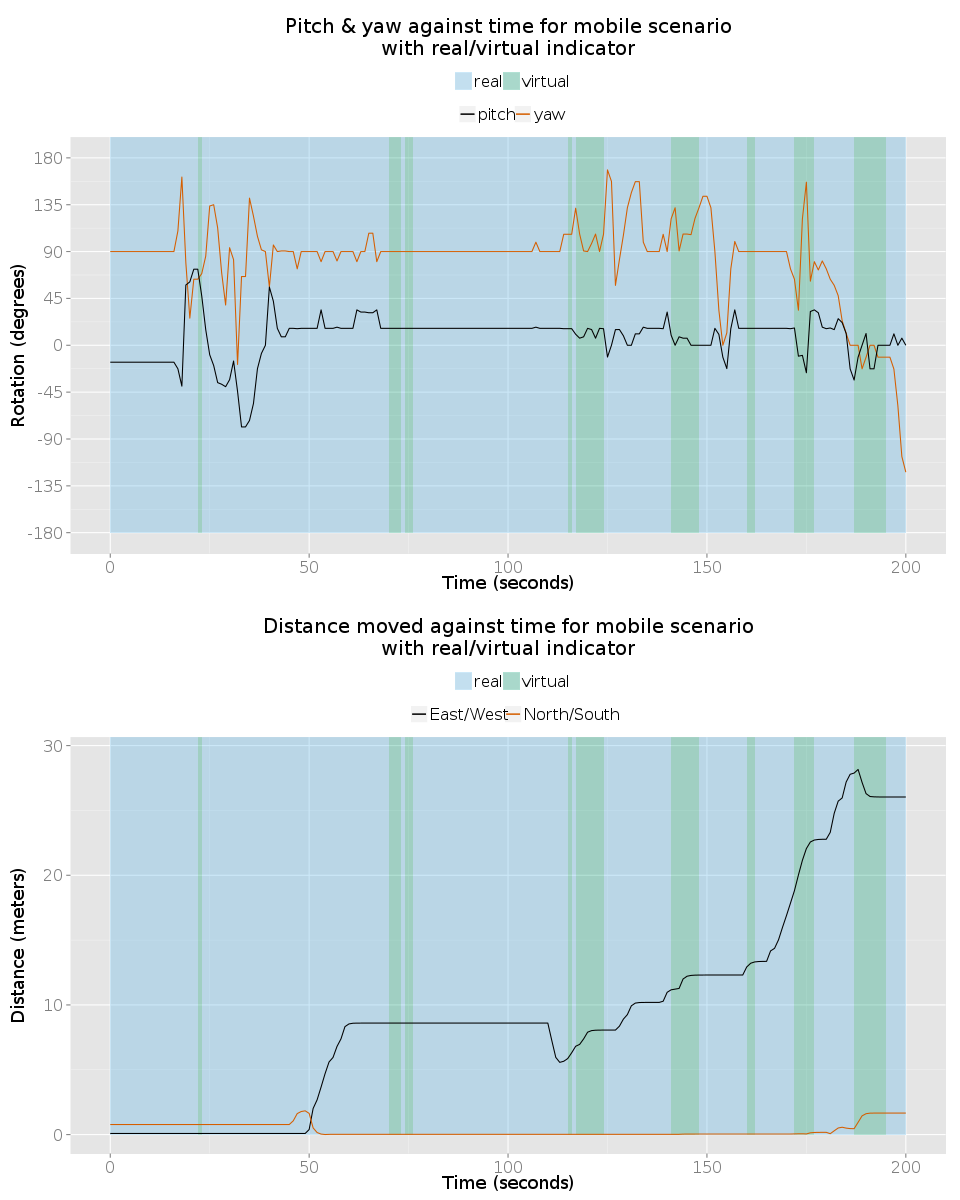
\includegraphics[width=\linewidth]{images/25072014_1400_2up.png}
		\caption{Participant 3}
		\label{participant_3_2up}
	\end{center}
\end{figure}

%=========================================================================================================

\begin{figure}[h]
	\begin{center}
		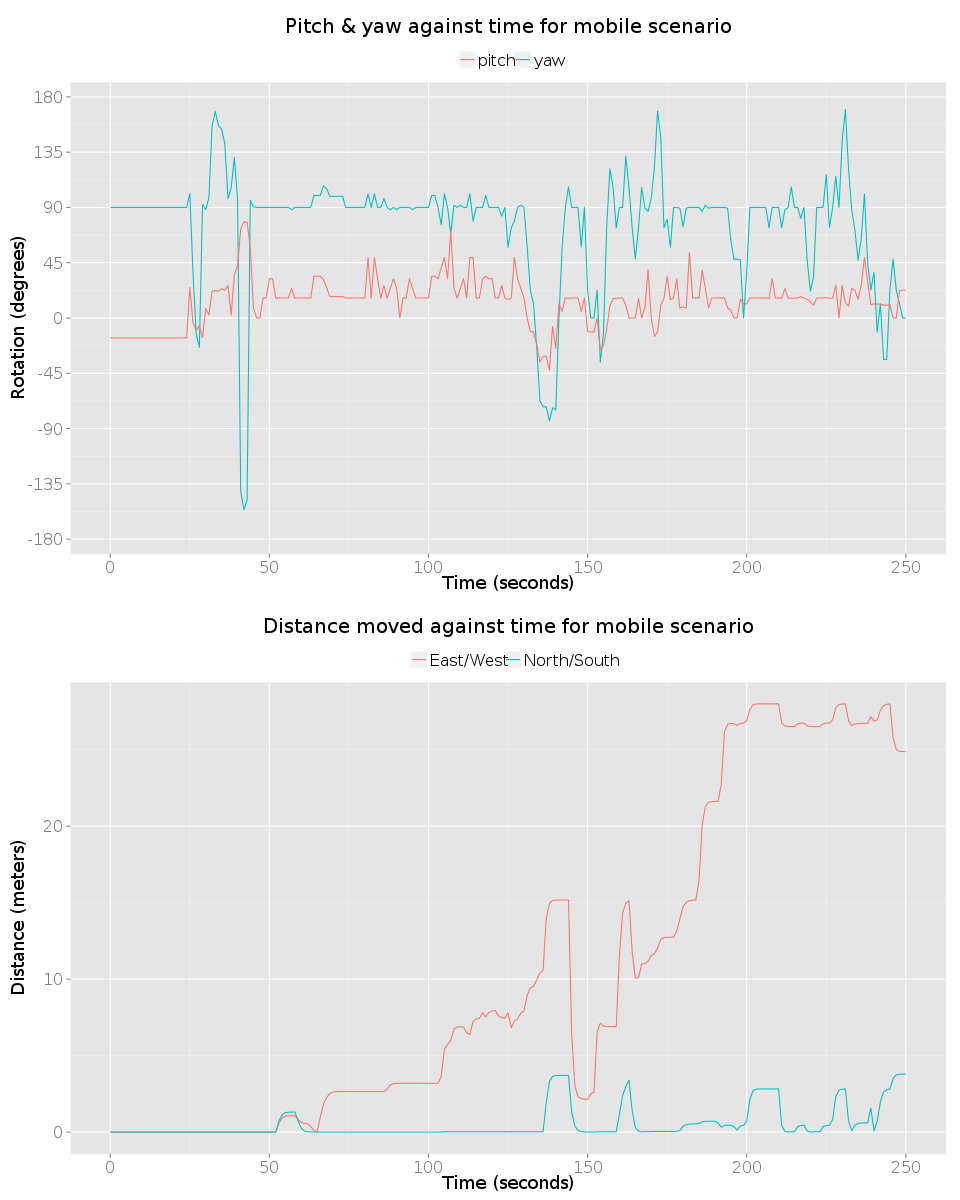
\includegraphics[width=\linewidth]{images/25072014_1500_4up.png}
		\caption{Participant 4}
		\label{participant_4_4up}
	\end{center}
\end{figure}

\begin{figure}[h]
	\begin{center}
		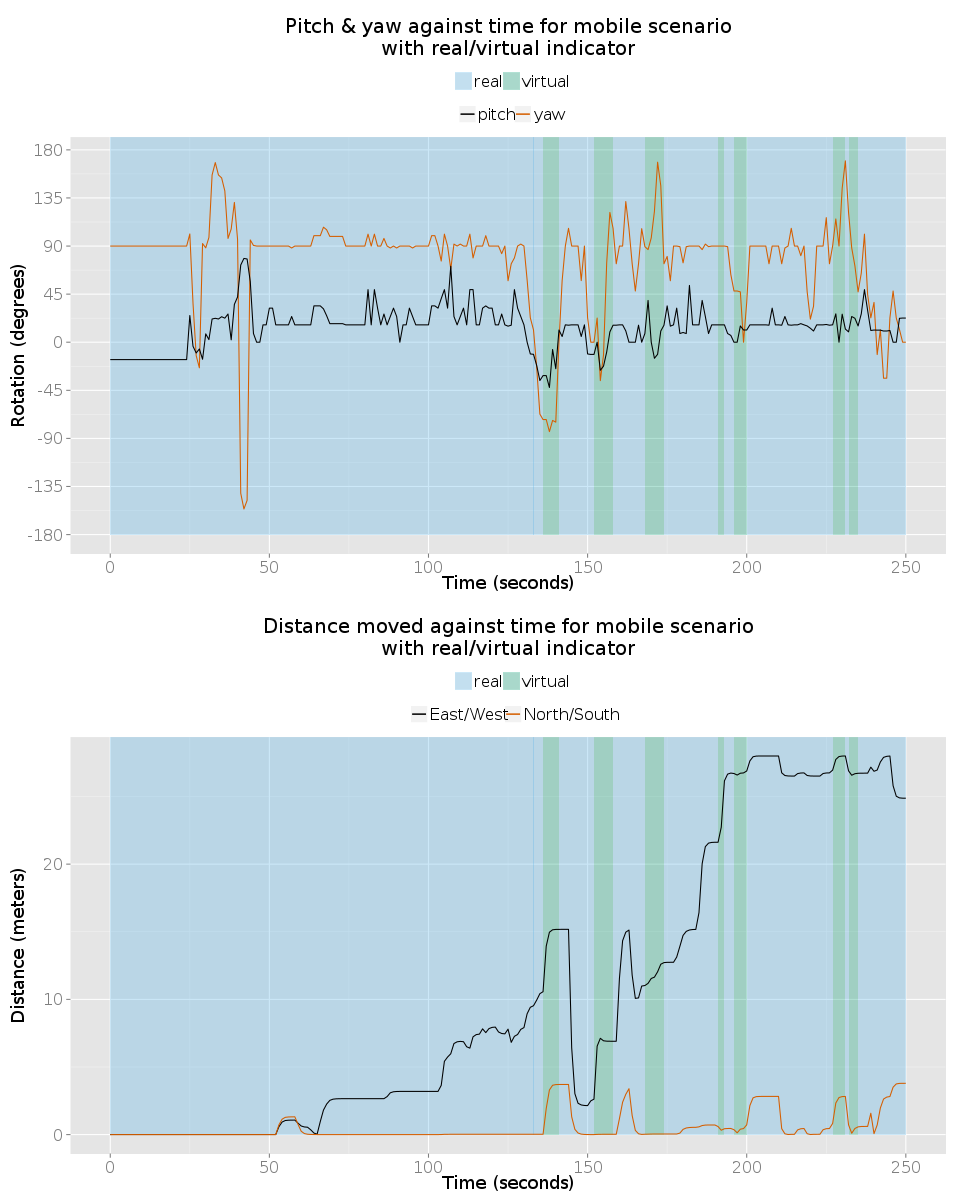
\includegraphics[width=\linewidth]{images/25072014_1500_2up.png}
		\caption{Participant 4}
		\label{participant_4_2up}
	\end{center}
\end{figure}

%=========================================================================================================

\begin{landscape}
	\begin{figure}[h]
		\begin{center}
			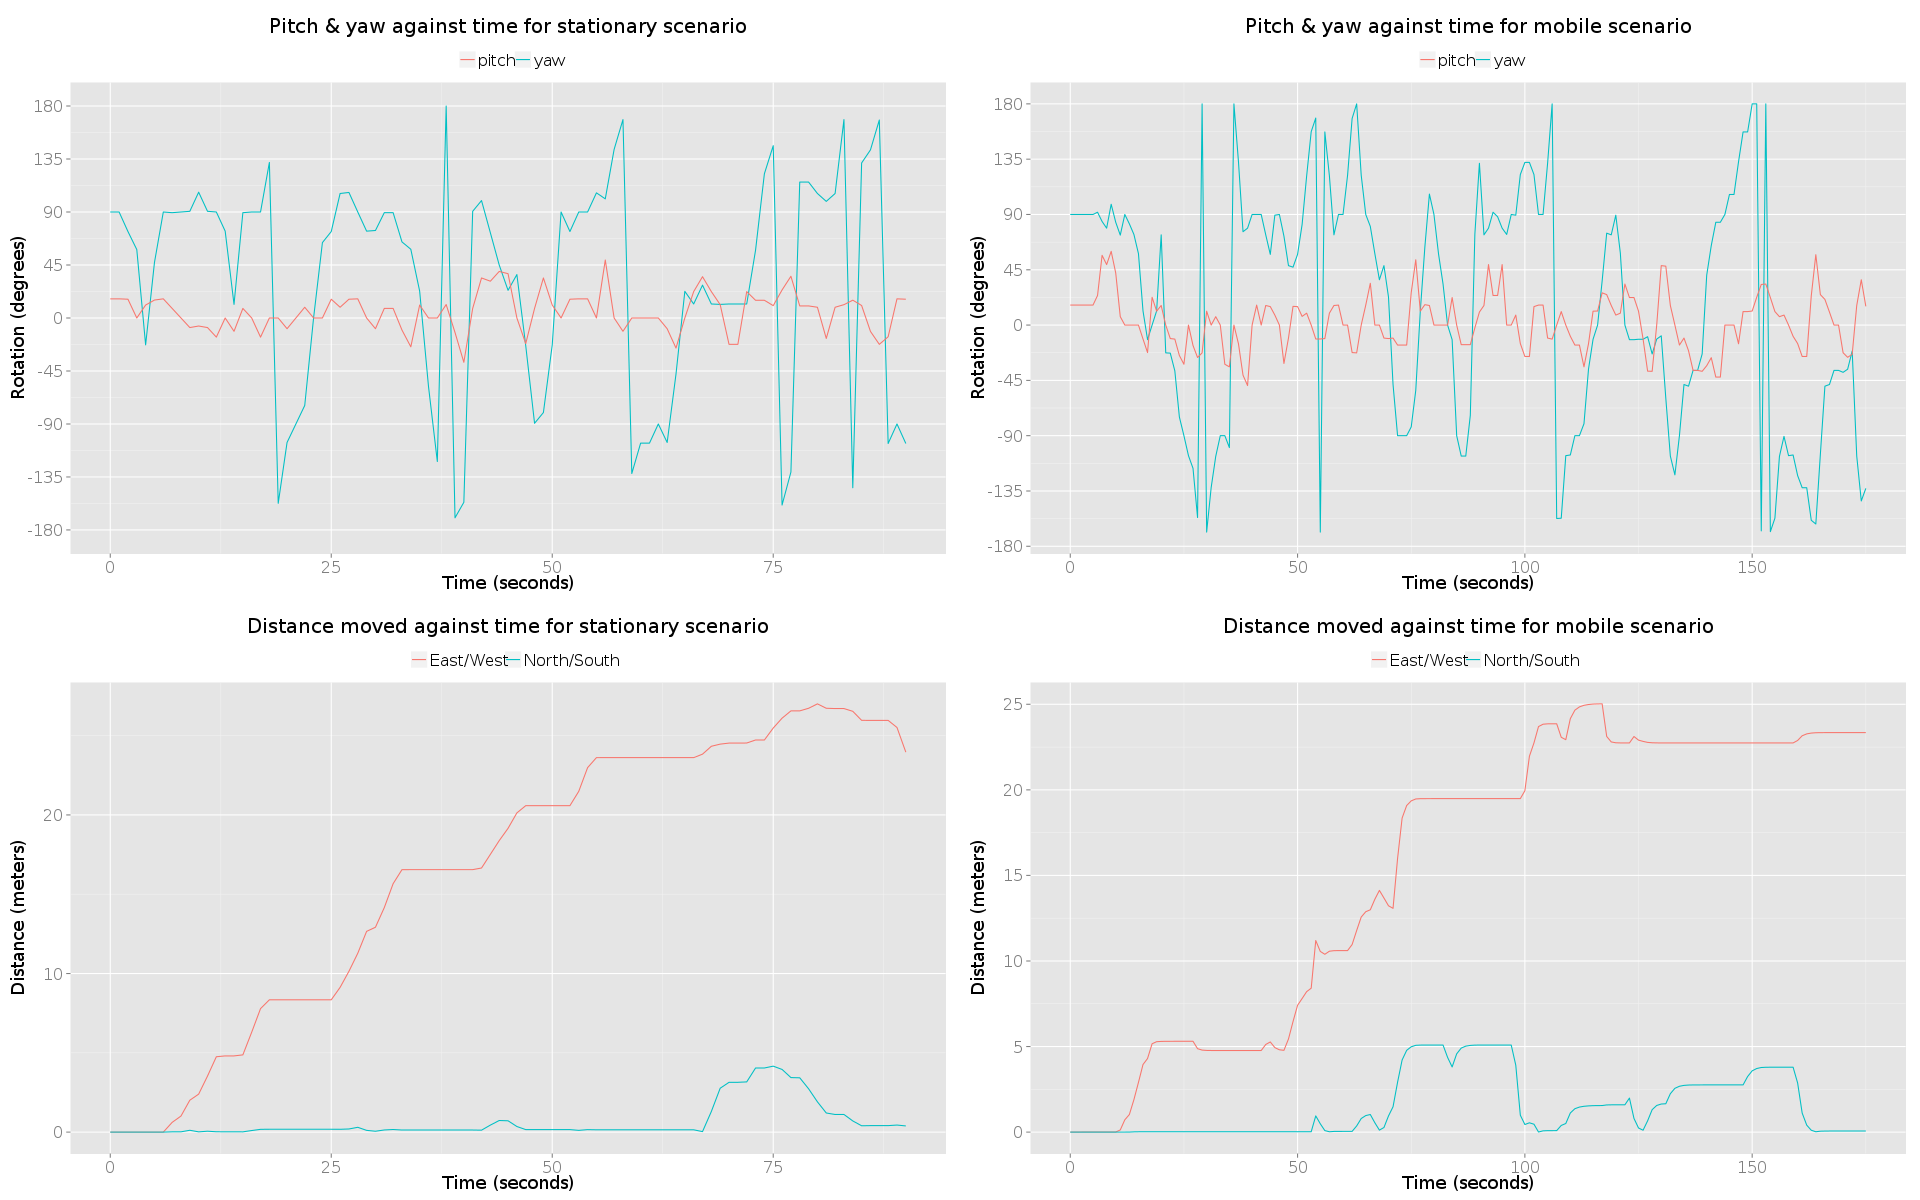
\includegraphics[width=\linewidth]{images/29082014_1350_4up.png}
			\caption{Participant 5}
			\label{participant_5_4up}
		\end{center}
	\end{figure}
\end{landscape}

\begin{figure}[h]
	\begin{center}
		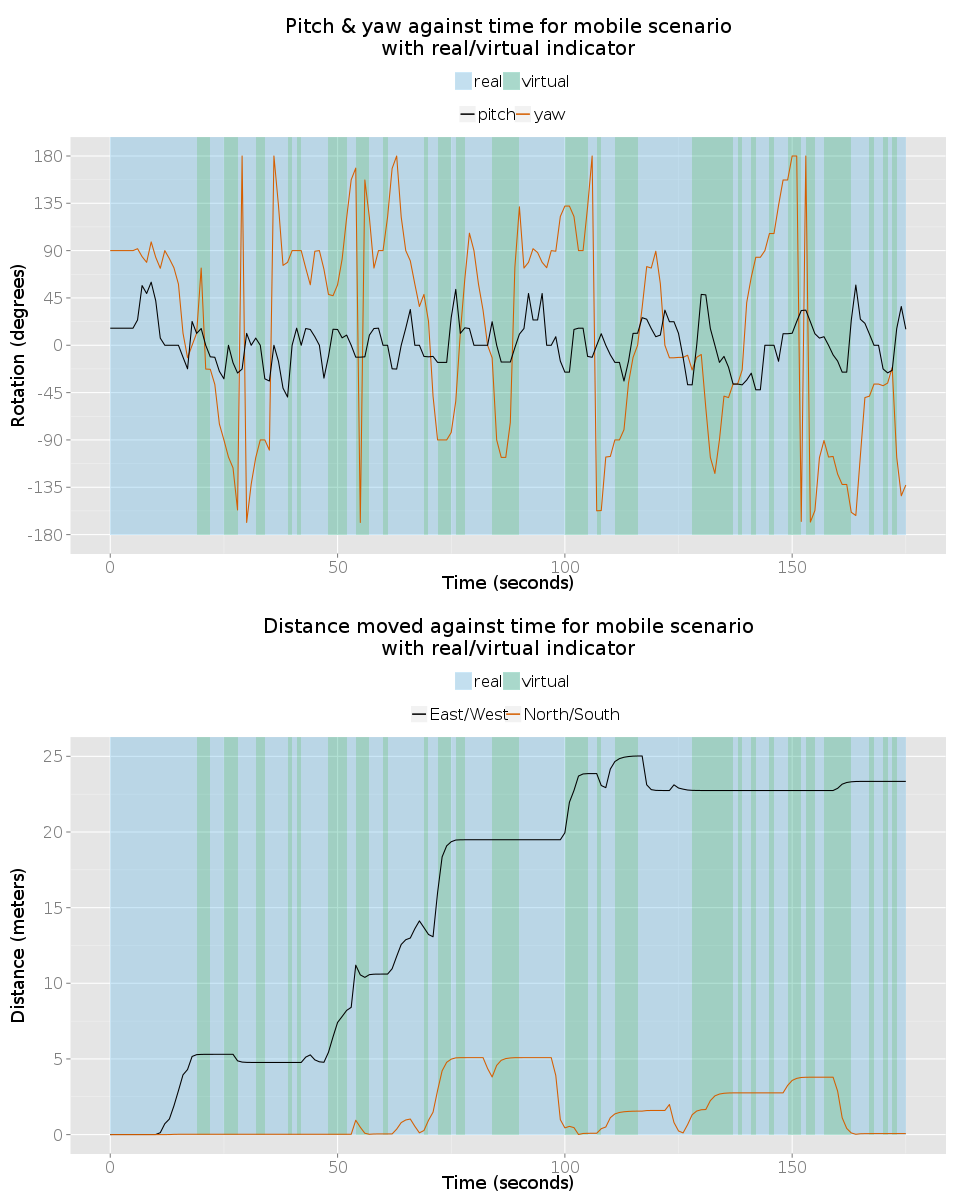
\includegraphics[width=\linewidth]{images/29082014_1350_2up.png}
		\caption{Participant 5}
		\label{participant_5_2up}
	\end{center}
\end{figure}

%=========================================================================================================

\pagebreak

\subsection{Interviews}

%=========================================================================================================

\bibliographystyle{unsrt}
\bibliography{bib}

\appendix
\chapter{Pre Task Questionnaire}
\label{pre_task_questionnaire}
\begin{figure}[h]
	\begin{center}
		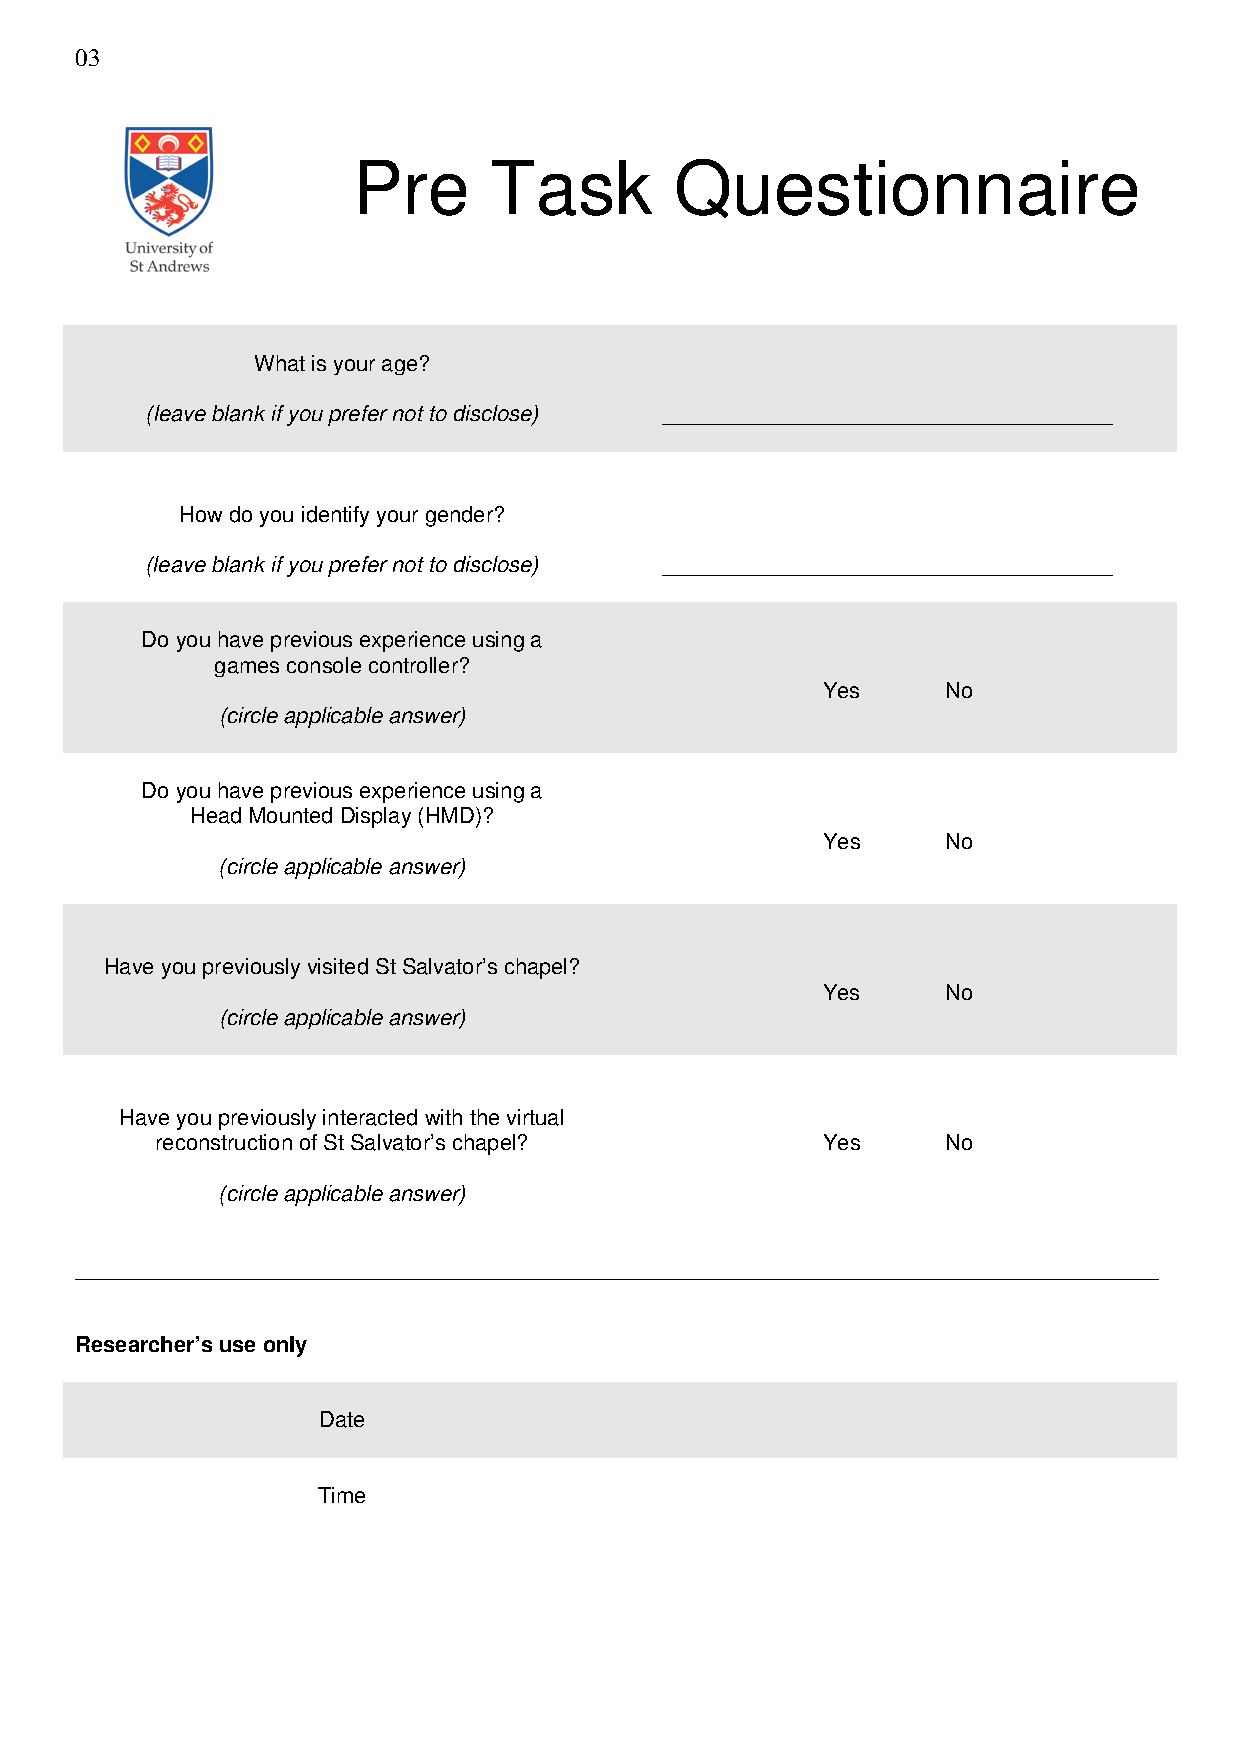
\includegraphics[width=0.7\linewidth]{PDFs/Pre_Task_Questionnaire.pdf}
	\end{center}
\end{figure}

\chapter{Post Task Questionnaire (SUS)}
\label{sus}
\begin{figure}[h]
	\begin{center}
		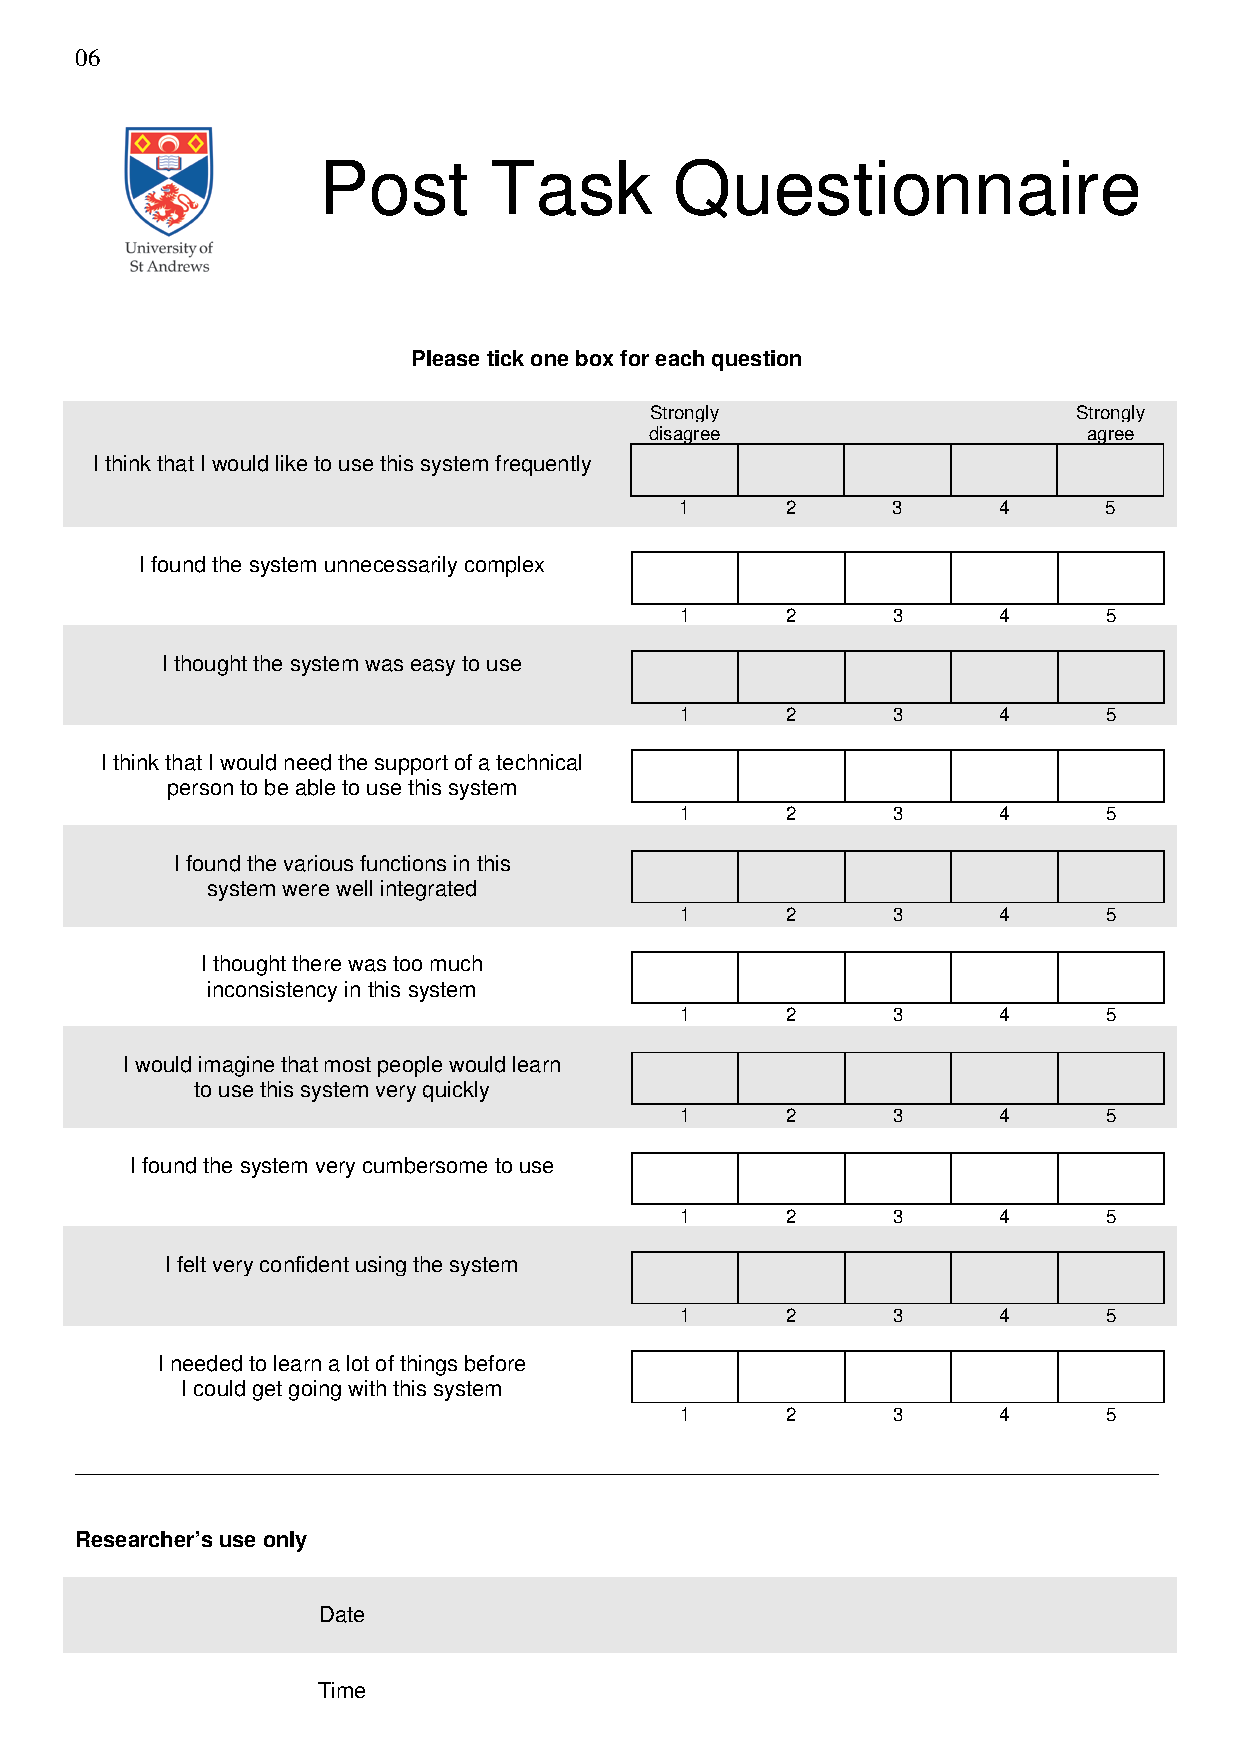
\includegraphics[width=0.7\linewidth]{PDFs/Post_Task_Questionnaire.pdf}
	\end{center}
\end{figure}

\chapter{Post Task Questionnaire (Own)}
\label{12_questions}
\begin{figure}[h]
	\begin{center}
		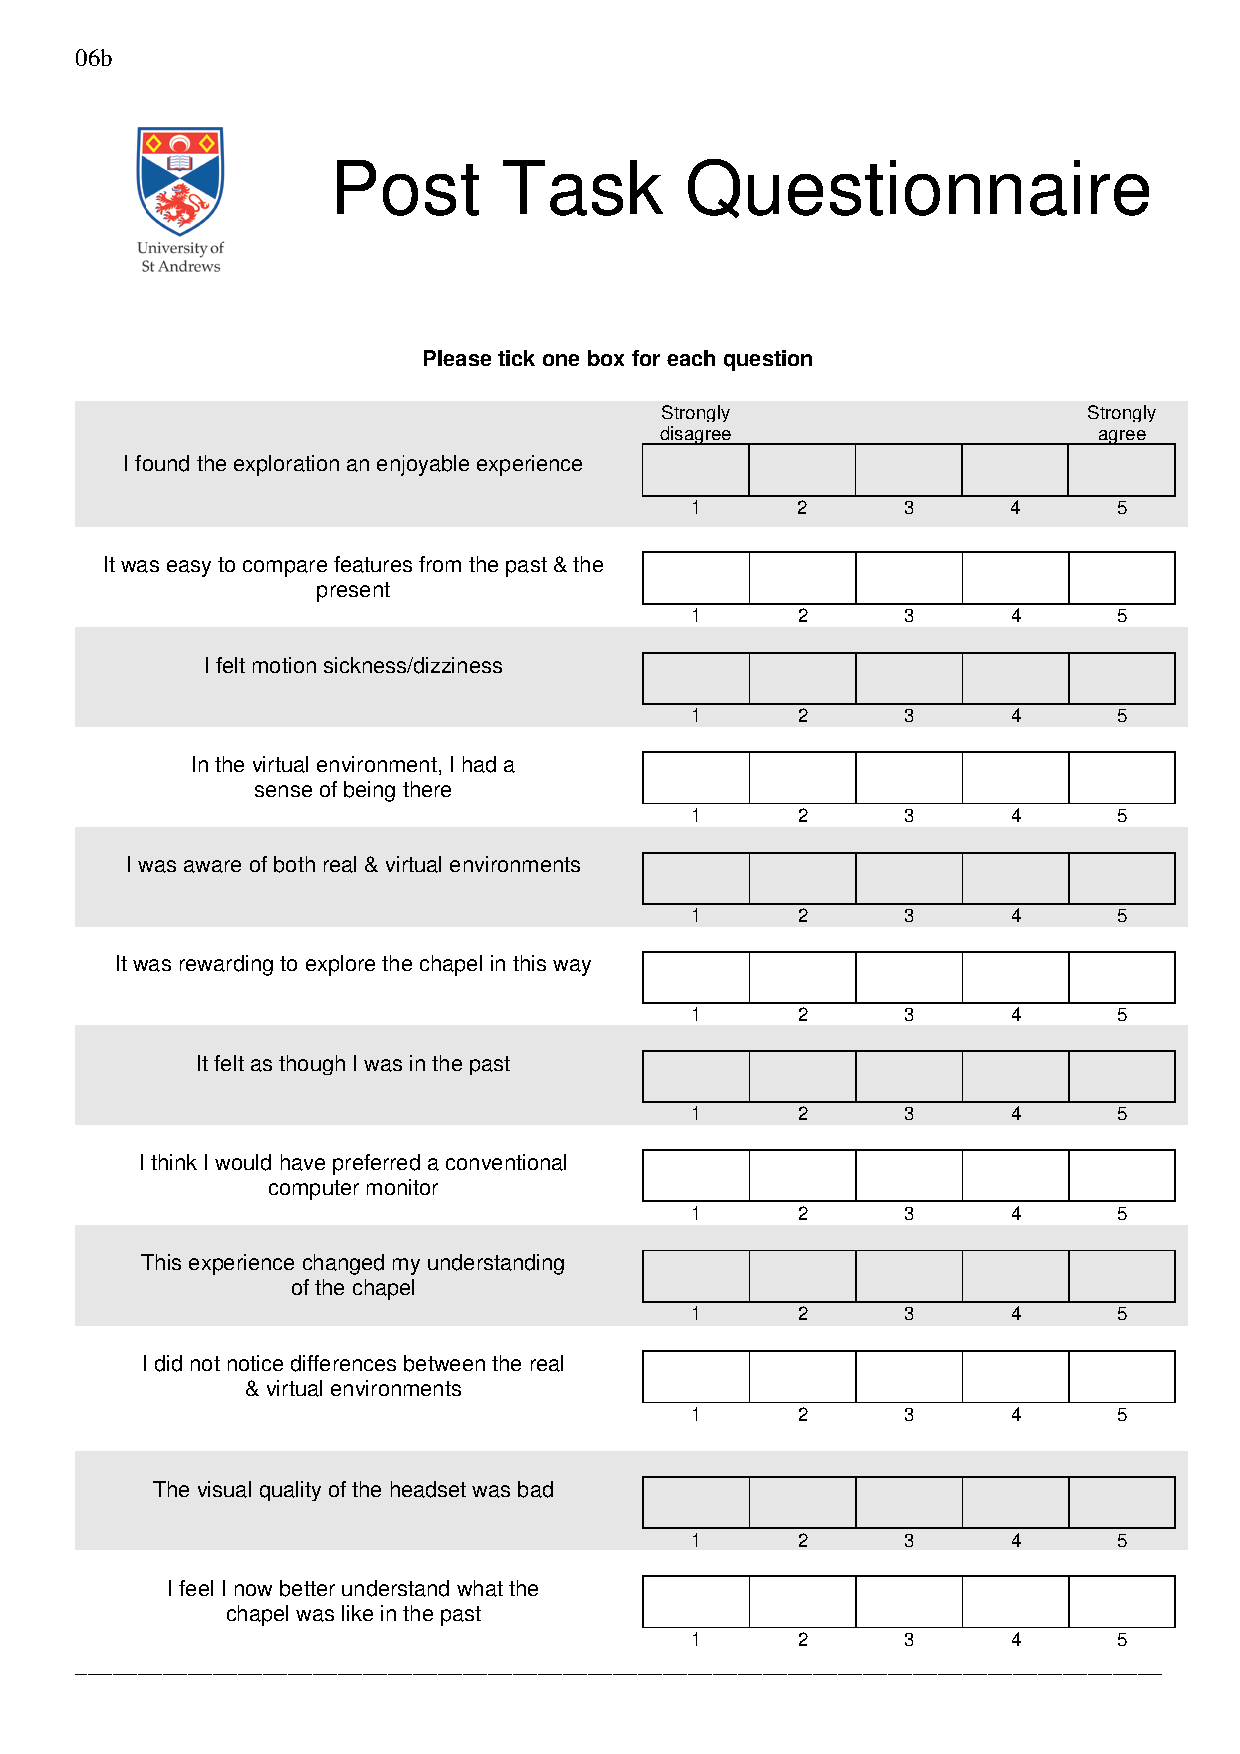
\includegraphics[width=0.7\linewidth]{PDFs/Post_Task_Questionnaire_2.pdf}
	\end{center}
\end{figure}

\chapter{Structured Interview Questions}
\label{interview_questions}
\begin{figure}[h]
	\begin{center}
		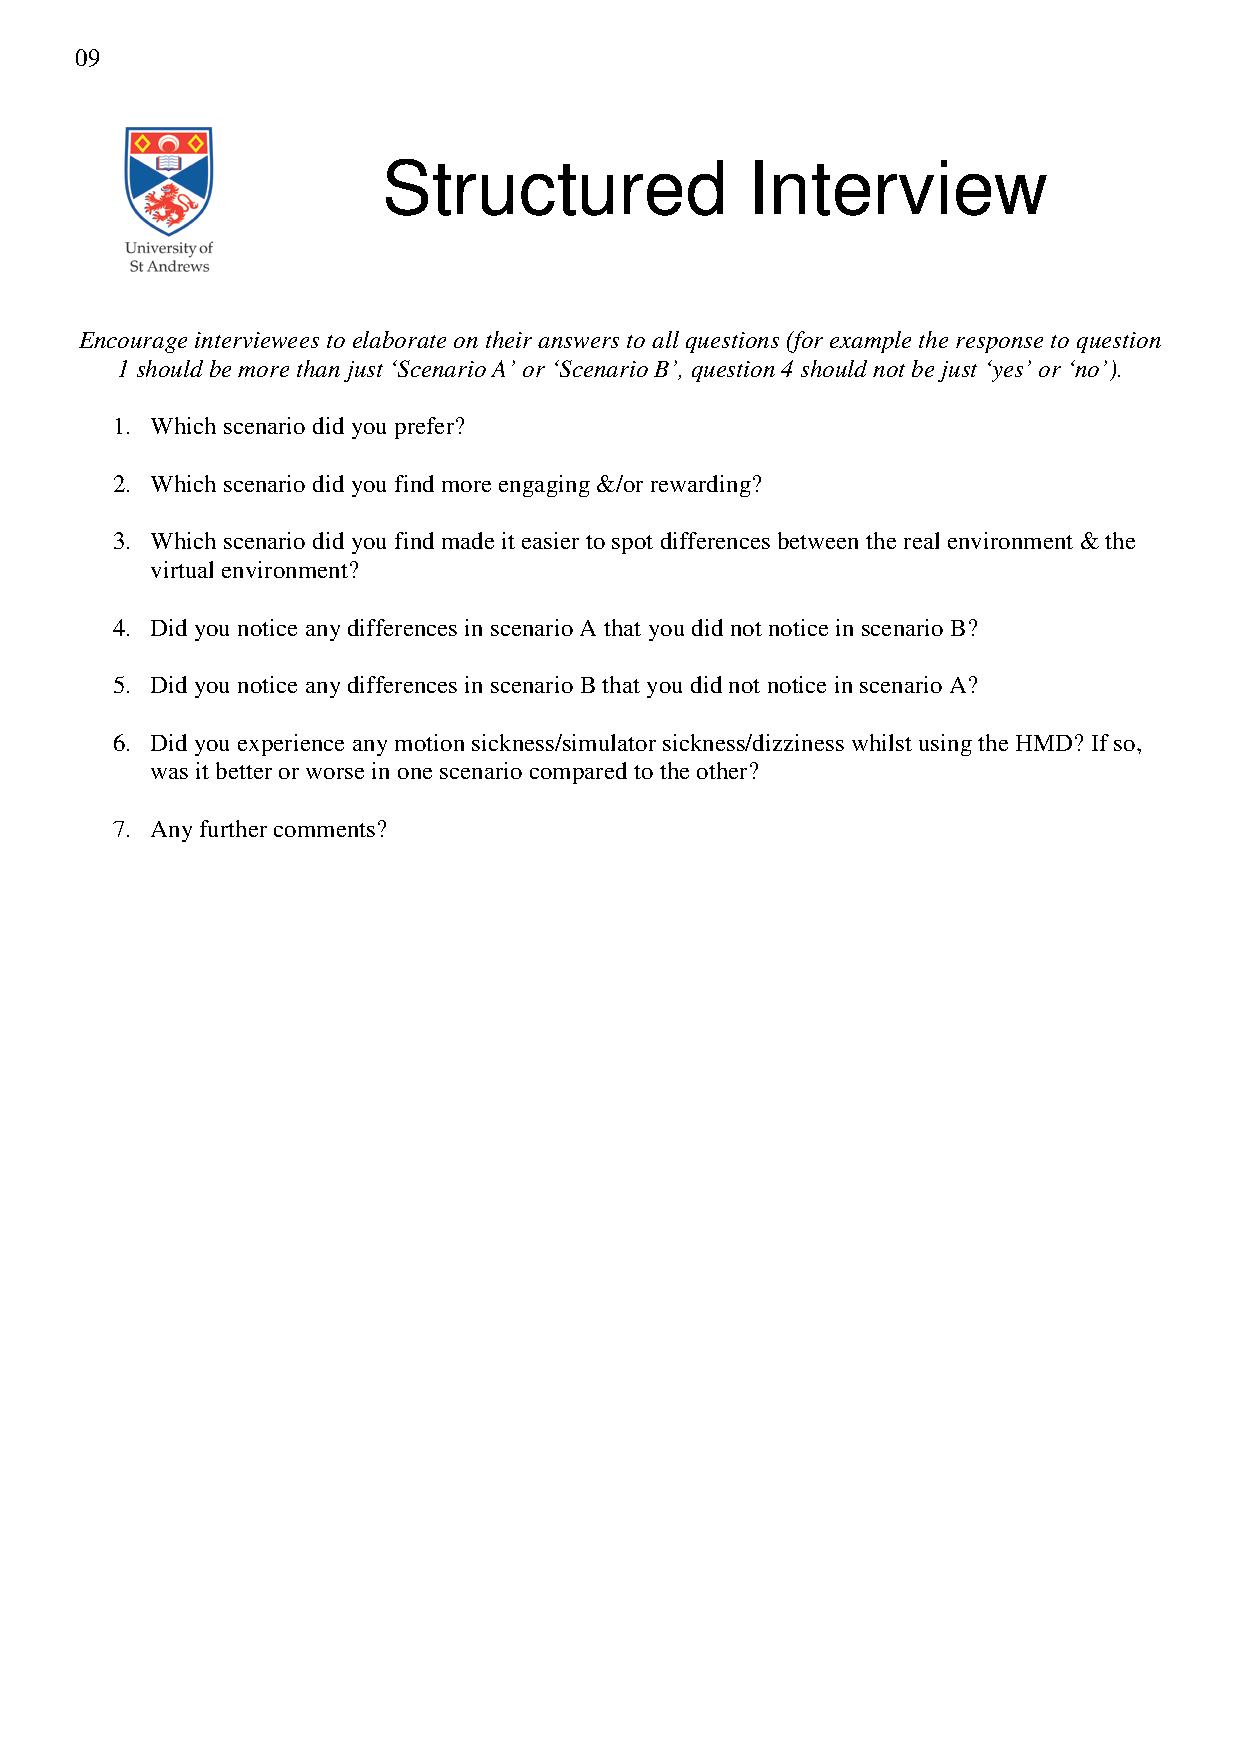
\includegraphics[width=0.7\linewidth]{PDFs/Structured_Interview.pdf}
	\end{center}
\end{figure}

\end{document}